% Options for packages loaded elsewhere
\PassOptionsToPackage{unicode}{hyperref}
\PassOptionsToPackage{hyphens}{url}
\PassOptionsToPackage{dvipsnames,svgnames,x11names}{xcolor}
\documentclass[
  11pt,
]{article}
\usepackage{xcolor}
\usepackage[margin=2.5cm]{geometry}
\usepackage{amsmath,amssymb}
\setcounter{secnumdepth}{-\maxdimen} % remove section numbering
\usepackage{iftex}
\ifPDFTeX
  \usepackage[T1]{fontenc}
  \usepackage[utf8]{inputenc}
  \usepackage{textcomp} % provide euro and other symbols
\else % if luatex or xetex
  \usepackage{unicode-math} % this also loads fontspec
  \defaultfontfeatures{Scale=MatchLowercase}
  \defaultfontfeatures[\rmfamily]{Ligatures=TeX,Scale=1}
\fi
\usepackage[]{charter}
\ifPDFTeX\else
  % xetex/luatex font selection
\fi
% Use upquote if available, for straight quotes in verbatim environments
\IfFileExists{upquote.sty}{\usepackage{upquote}}{}
\IfFileExists{microtype.sty}{% use microtype if available
  \usepackage[]{microtype}
  \UseMicrotypeSet[protrusion]{basicmath} % disable protrusion for tt fonts
}{}
\makeatletter
\@ifundefined{KOMAClassName}{% if non-KOMA class
  \IfFileExists{parskip.sty}{%
    \usepackage{parskip}
  }{% else
    \setlength{\parindent}{0pt}
    \setlength{\parskip}{6pt plus 2pt minus 1pt}}
}{% if KOMA class
  \KOMAoptions{parskip=half}}
\makeatother
\usepackage{graphicx}
\makeatletter
\newsavebox\pandoc@box
\newcommand*\pandocbounded[1]{% scales image to fit in text height/width
  \sbox\pandoc@box{#1}%
  \Gscale@div\@tempa{\textheight}{\dimexpr\ht\pandoc@box+\dp\pandoc@box\relax}%
  \Gscale@div\@tempb{\linewidth}{\wd\pandoc@box}%
  \ifdim\@tempb\p@<\@tempa\p@\let\@tempa\@tempb\fi% select the smaller of both
  \ifdim\@tempa\p@<\p@\scalebox{\@tempa}{\usebox\pandoc@box}%
  \else\usebox{\pandoc@box}%
  \fi%
}
% Set default figure placement to htbp
\def\fps@figure{htbp}
\makeatother
\setlength{\emergencystretch}{3em} % prevent overfull lines
\providecommand{\tightlist}{%
  \setlength{\itemsep}{0pt}\setlength{\parskip}{0pt}}
% ==========================================================================
%  IA na Sociedade — cabeçalho LaTeX (pdflatex)
%  Programa CiberExt 26-29 · FEELT38103
%  Adaptado de "AI in Society" (Universidade de Helsinque / Una Europa)
%  Licença: CC BY-NC-SA 4.0
% --------------------------------------------------------------------------
%  Espelha a identidade do ia-style.css: papel quente, tinta ardósia e a
%  faixa tricolor dos três eixos do curso (conceitos / aplicações / riscos).
% ==========================================================================

% ---------- Fontes ----------
% A serifada vem do build.sh, que passa  -V fontfamily=charter  ao pandoc.
% Aqui só acrescentamos a sem-serifa; ambas com fallback, porque nem toda
% instalação de LaTeX traz os mesmos pacotes.
\IfFileExists{helvet.sty}{\usepackage[scaled=0.90]{helvet}}{}
\usepackage{textcomp}
\IfFileExists{microtype.sty}{\usepackage{microtype}}{}

% ---------- Pacotes de layout ----------
\usepackage{xcolor}
\usepackage{tcolorbox}
\tcbuselibrary{skins,breakable}
\usepackage{titlesec}
\usepackage{fancyhdr}
\usepackage{enumitem}
\usepackage{amssymb}
\usepackage{booktabs}
\usepackage{array}
\usepackage{colortbl}
\usepackage{ragged2e}
\usepackage{fvextra}
\usepackage{newunicodechar}

% ---------- Caracteres Unicode que o pdflatex não conhece ----------
\newunicodechar{✓}{{\color{iaAplic}\checkmark}}
\newunicodechar{✅}{{\color{iaAplic}\checkmark}}
\newunicodechar{→}{\ensuremath{\rightarrow}}
\newunicodechar{←}{\ensuremath{\leftarrow}}
\newunicodechar{↔}{\ensuremath{\leftrightarrow}}
\newunicodechar{–}{--}
\newunicodechar{—}{---}
\newunicodechar{€}{\texteuro}
\newunicodechar{£}{\textsterling}
\newunicodechar{×}{\ensuremath{\times}}
\newunicodechar{≈}{\ensuremath{\approx}}
\newunicodechar{≥}{\ensuremath{\geq}}
\newunicodechar{≤}{\ensuremath{\leq}}
\newunicodechar{•}{\textbullet}
\newunicodechar{″}{''}
\newunicodechar{′}{'}

% ==========================================================================
%  PALETA — os mesmos valores do ia-style.css
% ==========================================================================
\definecolor{iaConceitos}{HTML}{24505C}   % petróleo — títulos, eixo 1
\definecolor{iaAplic}{HTML}{16746C}       % verdete  — subtítulos, eixo 2
\definecolor{iaRiscos}{HTML}{B45F14}      % açafrão  — destaques, eixo 3
\definecolor{iaAmeixa}{HTML}{77345F}      % links internos, termos técnicos
\definecolor{iaTinta}{HTML}{1F2933}       % corpo do texto
\definecolor{iaTintaFraca}{HTML}{5C6670}
\definecolor{iaRegra}{HTML}{E4DBCD}
\definecolor{iaBloco}{HTML}{F3EEE4}
\definecolor{iaNota}{HTML}{EAF1F0}
\definecolor{iaCaso}{HTML}{FCF3E6}
\definecolor{iaFilos}{HTML}{F7EFF4}

\color{iaTinta}

% ==========================================================================
%  ASSINATURA — faixa tricolor dos três eixos
% ==========================================================================
\newcommand{\faixaEixos}[1][\linewidth]{%
  \noindent
  \textcolor{iaConceitos}{\rule{0.3333#1}{4pt}}%
  \textcolor{iaAplic}{\rule{0.3333#1}{4pt}}%
  \textcolor{iaRiscos}{\rule{0.3333#1}{4pt}}%
  \par}

% ---------- Página de título ----------
\makeatletter
\newcommand{\subtitle}[1]{\gdef\@subtitle{#1}}
\providecommand{\@subtitle}{}
\def\@maketitle{%
  \newpage\null\vskip 1.5em%
  \faixaEixos
  \vskip 2.2em
  {\raggedright
    {\sffamily\bfseries\huge\color{iaConceitos}\@title\par}%
    \vskip 0.7em%
    {\sffamily\large\color{iaTintaFraca}\@subtitle\par}%
    \vskip 2em%
    {\color{iaRegra}\rule{\linewidth}{1pt}}%
    \vskip 1em%
    {\sffamily\small\color{iaTinta}\@author\par}%
    \vskip 0.5em%
    {\sffamily\footnotesize\color{iaTintaFraca}\@date\par}%
  }\par\vskip 2.5em}
\makeatother

% ==========================================================================
%  TÍTULOS DE SEÇÃO
% ==========================================================================
\titleformat{\section}[block]
  {\sffamily\Large\bfseries\color{iaConceitos}}
  {\thesection}{0.7em}{}
  [{\vspace{2pt}\color{iaRegra}\titlerule[1.2pt]}]
\titleformat{\subsection}
  {\sffamily\large\bfseries\color{iaAplic}}
  {\thesubsection}{0.6em}{}
\titleformat{\subsubsection}
  {\sffamily\normalsize\bfseries\color{iaRiscos}}
  {\thesubsubsection}{0.5em}{}
\titleformat{\paragraph}[runin]
  {\sffamily\small\bfseries\color{iaRiscos}}
  {}{0em}{}

\titlespacing*{\section}{0pt}{2.6ex plus 1ex minus .2ex}{1.3ex plus .2ex}
\titlespacing*{\subsection}{0pt}{2.2ex plus 1ex minus .2ex}{1ex plus .2ex}

% ==========================================================================
%  CABEÇALHO E RODAPÉ
% ==========================================================================
\setlength{\headheight}{24pt}
\renewcommand{\sectionmark}[1]{\markboth{#1}{}}
\pagestyle{fancy}
\fancyhf{}
\renewcommand{\headrulewidth}{0.6pt}
\renewcommand{\footrulewidth}{0pt}
\fancyhead[L]{\sffamily\footnotesize\color{iaAplic}Ética da IA}
\fancyhead[R]{\sffamily\footnotesize\color{iaAplic}\nouppercase{\leftmark}}
\fancyfoot[C]{\sffamily\footnotesize\color{iaConceitos}\thepage}
\renewcommand{\headrule}{%
  \hbox to\headwidth{\color{iaRegra}\leaders\hrule height \headrulewidth\hfill}}

% ==========================================================================
%  TEXTO CORRIDO
% ==========================================================================
\linespread{1.08}
\setlength{\parskip}{0.55em}
\setlength{\parindent}{0pt}
\emergencystretch=3em
\hbadness=10000

% ---------- Termos técnicos / código inline ----------
\let\oldtexttt\texttt
\renewcommand{\texttt}[1]{{\color{iaAmeixa}\small\ttfamily #1}}

% ---------- Blocos verbatim ----------
\fvset{breaklines=true,breakanywhere=true,fontsize=\small}

% ---------- Blocos de código (ambiente Shaded do pandoc) ----------
% O pandoc só pré-define o ambiente Shaded quando o markdown tem bloco de
% código; nos capítulos sem código ele não existe, e \renewenvironment
% incondicional falharia com "Environment Shaded undefined". \@ifundefined
% escolhe \newenvironment ou \renewenvironment conforme o caso.
\makeatletter
\@ifundefined{Shaded}{\newenvironment{Shaded}}{\renewenvironment{Shaded}}
  {\begin{tcolorbox}[
      breakable, enhanced jigsaw, rounded corners,
      arc=3pt, boxrule=0pt, frame hidden,
      colback=iaBloco,
      borderline west={3pt}{0pt}{iaAmeixa},
      left=10pt, right=8pt, top=6pt, bottom=6pt,
      before skip=9pt, after skip=9pt]}
  {\end{tcolorbox}}
\makeatother

% ---------- Citações: caixa de caso ----------
\renewenvironment{quote}
  {\begin{tcolorbox}[
      breakable, enhanced jigsaw, rounded corners,
      arc=3pt, boxrule=0pt, frame hidden,
      colback=iaCaso,
      borderline west={3pt}{0pt}{iaRiscos},
      left=12pt, right=10pt, top=9pt, bottom=9pt,
      before skip=9pt, after skip=9pt]}
  {\end{tcolorbox}}

% ==========================================================================
%  BLOCOS DE APOIO
%  No markdown, escreva:   ::: nota   ...texto...   :::
%  O pandoc converte fenced_divs para os ambientes abaixo.
% ==========================================================================
\newtcolorbox{iabox}[3]{
  breakable, enhanced jigsaw, rounded corners,
  arc=3pt, boxrule=0pt, frame hidden,
  colback=#2,
  borderline west={3pt}{0pt}{#1},
  left=12pt, right=10pt, top=9pt, bottom=9pt,
  before skip=11pt, after skip=11pt,
  before upper={\setlength{\parskip}{0.5em}\setlength{\parindent}{0pt}},
  title={\sffamily\bfseries\footnotesize\textcolor{#1}{\MakeUppercase{#3}}},
  attach title to upper={\par\vspace{5pt}},
  fonttitle=\normalfont}

% Cada ambiente aceita um titulo opcional entre colchetes, vindo do
% atributo data-titulo do markdown:   \begin{filosofia}[Titulo] ... \end{filosofia}
% Os quatro primeiros espelham os icones do material original.
\newenvironment{filosofia}[1][Conceito filosofico]{\begin{iabox}{iaAmeixa}{iaFilos}{#1}}{\end{iabox}}
\newenvironment{tecnica}[1][Nota tecnica]{\begin{iabox}{iaConceitos}{iaNota}{#1}}{\end{iabox}}
\newenvironment{contexto}[1][Contexto]{\begin{iabox}{iaAplic}{iaBloco}{#1}}{\end{iabox}}
\newenvironment{definicao}[1][Definicao]{\begin{iabox}{iaRiscos}{iaCaso}{#1}}{\end{iabox}}

\newenvironment{nota}[1][Nota]{\begin{iabox}{iaConceitos}{iaNota}{#1}}{\end{iabox}}
\newenvironment{caso}[1][Caso]{\begin{iabox}{iaRiscos}{iaCaso}{#1}}{\end{iabox}}
\newenvironment{reflexao}[1][Para pensar]{\begin{iabox}{iaAplic}{iaBloco}{#1}}{\end{iabox}}
\newenvironment{licenca}
  {\par\vspace{2em}\faixaEixos\par\vspace{0.8em}
   \begingroup\sffamily\scriptsize\color{iaTintaFraca}}
  {\endgroup\par}

% ==========================================================================
%  LISTAS
% ==========================================================================
\setlist[itemize]{leftmargin=1.4em, itemsep=2pt, topsep=4pt, parsep=0pt}
\setlist[enumerate]{leftmargin=1.7em, itemsep=2pt, topsep=4pt, parsep=0pt}
\renewcommand{\labelitemi}{\textcolor{iaRiscos}{\textbullet}}
\renewcommand{\labelitemii}{\textcolor{iaAplic}{--}}

% ==========================================================================
%  TABELAS
% ==========================================================================
\renewcommand{\arraystretch}{1.3}
\arrayrulecolor{iaRegra}

% ==========================================================================
%  RÓTULOS EM PORTUGUÊS
%  Definidos aqui (e não via -V na linha de comando) porque acentos passados
%  como argumento dependem do locale do terminal e podem se corromper.
% ==========================================================================
\renewcommand{\contentsname}{Sumário}
\renewcommand{\refname}{Referências}
\renewcommand{\figurename}{Figura}
\renewcommand{\tablename}{Tabela}
\usepackage{bookmark}
\IfFileExists{xurl.sty}{\usepackage{xurl}}{} % add URL line breaks if available
\urlstyle{same}
% fallback for those not using the hyperref driver hyperxmp:
\makeatletter
\@ifundefined{xmpquote}{\newcommand{\xmpquote}[1]{#1}}{}
\makeatother
\hypersetup{
  pdftitle={Ética da Inteligência Artificial},
  colorlinks=true,
  linkcolor={iaAmeixa},
  filecolor={Maroon},
  citecolor={Blue},
  urlcolor={iaRiscos},
  pdfcreator={LaTeX via pandoc}}

\title{Ética da Inteligência Artificial}
\usepackage{etoolbox}
\makeatletter
\providecommand{\subtitle}[1]{% add subtitle to \maketitle
  \apptocmd{\@title}{\par {\large #1 \par}}{}{}
}
\makeatother
\subtitle{Capítulo 6: Equidade --- a IA deve ser justa e não
discriminatória?}
\author{Tradução e adaptação para o português: José Lucas Lira Bizil,
Fernando Mazzeto Lisboa Lima e Matheus da Silva Fernandes\\
Programa CiberExt 26-29 · FEELT38103 · Universidade Federal de
Uberlândia\\
Original: \emph{Ethics of AI}, Universidade de Helsinque}
\date{2026}

\begin{document}
\maketitle

{
\hypersetup{linkcolor=iaConceitos}
\setcounter{tocdepth}{3}
\tableofcontents
}
\section{Capítulo 6: Equidade --- a IA deve ser justa e não
discriminatória?}\label{capuxedtulo-6-equidade-a-ia-deve-ser-justa-e-nuxe3o-discriminatuxf3ria}

\begin{nota}[Sobre este capítulo]

\textbf{Eixo:} Conceitos, Aplicações e Riscos

O que é justiça? O que distingue igualdade de equidade? Quando uma
diferença de tratamento se torna discriminação? Este capítulo examina os
danos alocativos e representacionais, as três origens do viés
(\emph{bias}) e por que ser justo não é o mesmo que ser ético.

\end{nota}

\subsection{I. O que é justiça?}\label{i.-o-que-uxe9-justiuxe7a}

\begin{definicao}[Experimento mental: o algoritmo das notas]

Para este experimento mental, suponhamos que, por causa da pandemia de
covid-19, todos os exames de conclusão do ensino médio finlandês tenham
sido cancelados. Em lugar do exame, seria preciso projetar e implementar
um método alternativo para determinar as notas de qualificação
atribuídas aos estudantes naquele ano. Como os estudantes são admitidos
na universidade com base em suas notas, as notas desses exames são
extremamente importantes.

O governo decidiu que os professores dariam uma estimativa de como
achavam que seus alunos teriam se saído nos exames, e que isso
determinaria as notas. Pediu- se aos professores que fizessem avaliações
de seus alunos.

Para combater a inflação de notas, foi usado um algoritmo que ponderava
as pontuações com base no desempenho histórico de cada escola. A ideia
era que o algoritmo compensasse a tendência dos professores a inflar o
desempenho esperado de seus alunos e que, assim, as estimativas
previssem com mais exatidão como os examinandos teriam de fato se saído.
O algoritmo foi projetado com duas informações: a posição do aluno
dentro da escola e o desempenho histórico da escola.

Como resultado, em nível nacional as notas corresponderam razoavelmente
bem à distribuição de notas dos anos anteriores. No entanto, o algoritmo
rebaixou quase 40\% das notas previstas pelos professores. Os dados
mostraram que os resultados de estudantes de origem socioeconômica mais
baixa foram rebaixados com mais frequência do que os de origem
socioeconômica mais alta. Para estudantes de baixa renda que esperavam
ir para a universidade, os resultados foram devastadores.

\end{definicao}

Muitos tomariam este experimento mental como exemplo de injustiça
algorítmica. Ele não descreve apenas como algoritmos podem, por si,
produzir resultados injustos, mas também como podem reforçar vieses
econômicos e sociais já existentes.

\subsubsection{Justiça e viés}\label{justiuxe7a-e-viuxe9s}

Justiça e viés são provavelmente as questões éticas mais discutidas em
relação aos algoritmos contemporâneos. Por que são tão centrais?

\begin{itemize}
\item
  \textbf{Primeiro}, a justiça é elemento fundamental da estabilidade
  social. Como observa o filósofo John Rawls, a estabilidade de uma
  sociedade --- ou de qualquer grupo --- depende da medida em que seus
  membros sentem que estão sendo tratados de maneira justa. Quando
  alguns membros sentem que são tratados de modo injusto, isso costuma
  criar a base para inquietação social, distúrbios e conflito. As
  pessoas mantêm a unidade social apenas na medida em que suas
  instituições são justas.
\item
  \textbf{Segundo}, como observou Immanuel Kant, os seres humanos têm a
  mesma dignidade. Em virtude dessa dignidade, têm direito a ser
  tratados como iguais. Se indivíduos são tratados injustamente ---
  especialmente por motivos arbitrários ---, sua dignidade humana
  fundamental é violada. Quando essa violação se efetiva em práticas,
  leva à discriminação.
\end{itemize}

Contudo, como ilustra o exemplo do algoritmo de inflação de notas, a
justiça é uma questão complexa. O algoritmo foi projetado para corrigir
a inflação de notas porque se julgava injusto que estudantes obtivessem
vantagem indevida. Como resultado, paradoxalmente, o algoritmo acabou
reforçando vieses sociais já existentes.

Neste capítulo, vamos nos concentrar em justiça, vieses e discriminação.
Abordaremos questões como: o que exatamente é justiça? A justiça deve
consistir em assegurar que todos tenham probabilidade igual de obter
algum benefício? Ou deve levar em conta as diferenças individuais e
reconhecer a diversidade? E, por fim: justiça e discriminação são
sinônimos, ou significam coisas distintas?

\subsection{II. As variedades da
justiça}\label{ii.-as-variedades-da-justiuxe7a}

Filósofos propuseram várias definições para o conceito de justiça.
Segundo Aristóteles, ``os iguais devem ser tratados igualmente, e os
desiguais, desigualmente''.

Esse \textbf{princípio da igualdade} afirma que os indivíduos devem ser
tratados da mesma forma, a menos que difiram de maneiras relevantes para
a situação em que estão envolvidos.

Por exemplo, se Alan Turing e Ada Lovelace obtiveram as mesmas notas nos
exames e não há diferenças relevantes entre eles ou entre os exames que
prestaram, então devem receber a mesma nota. E se Turing recebesse nota
melhor do que Lovelace simplesmente por ter status socioeconômico mais
alto, isso seria injusto. Por quê? Porque o status socioeconômico não
deveria ser relevante na atribuição de notas.

Contudo, o princípio da igualdade foi criticado por ser ``cego''. Ele
não leva em conta que nem todos partimos da mesma posição, nem que
existem diferenças individuais que importam. Em contraste com a
igualdade, a ``equidade'' não promove justiça tratando categoricamente
todos do mesmo modo, e sim dando a todos acesso igual às mesmas
oportunidades. Há situações, por exemplo, em que a diferença de origem
socioeconômica é critério relevante para tratar as pessoas de modo
distinto. A maioria das pessoas considerou justo, por exemplo, que o
governo conceda benefícios sociais apenas aos cidadãos que realmente
precisam, e não a todos.

\textbf{Igualdade} significa que todos são tratados da mesma forma.

\begin{figure}
\centering
\pandocbounded{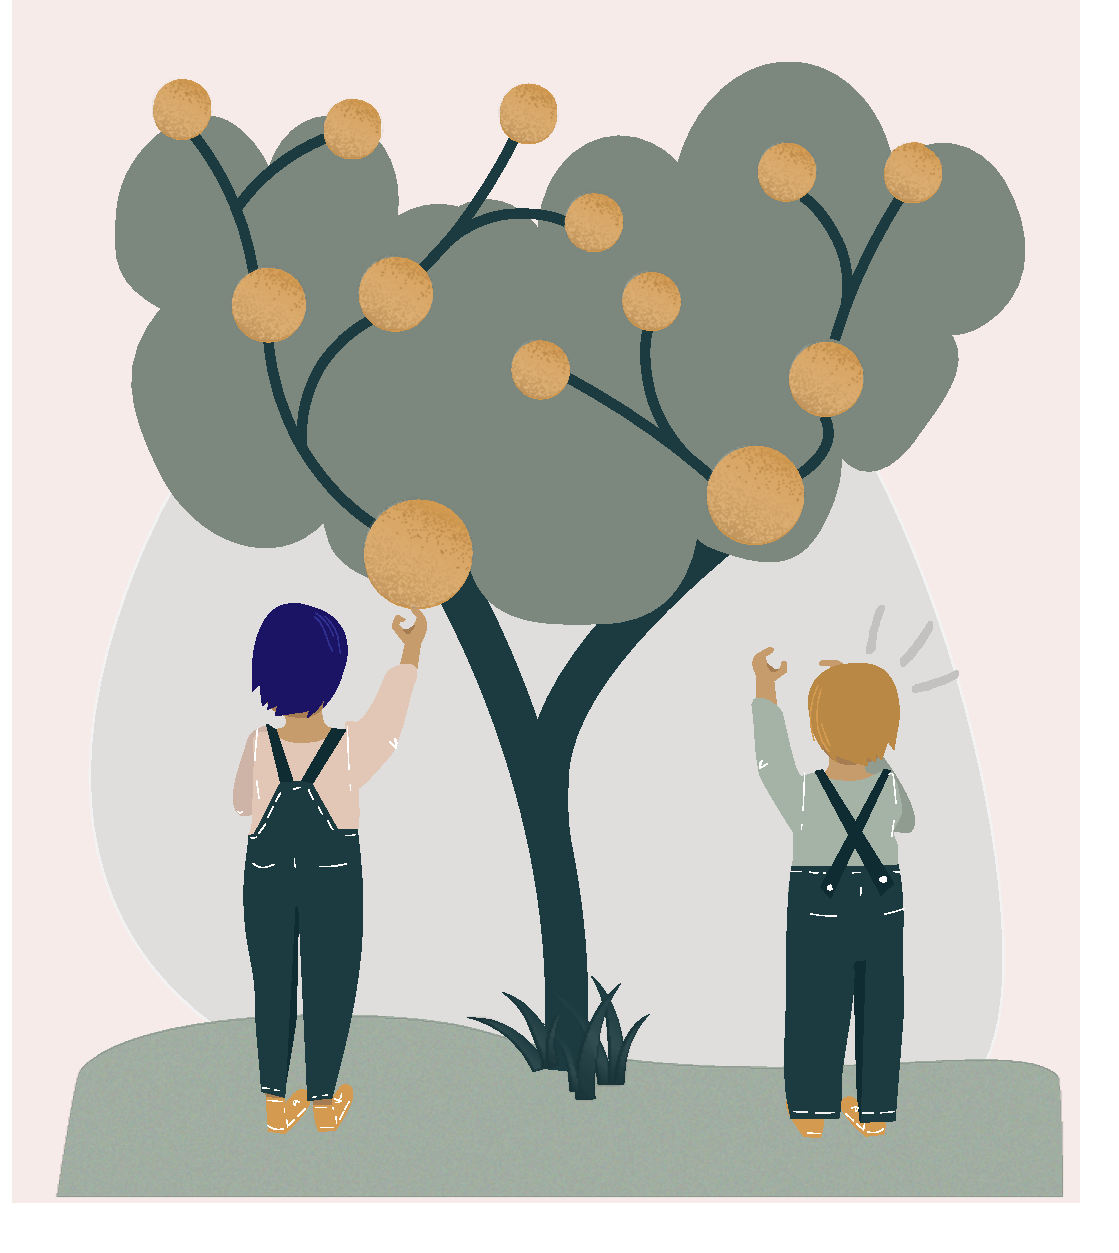
\includegraphics[keepaspectratio,alt={Igualdade}]{img/equality.pdf}}
\caption{Igualdade}
\end{figure}

\textbf{Equidade} significa que cada um recebe o que precisa para ter
sucesso.

\begin{figure}
\centering
\pandocbounded{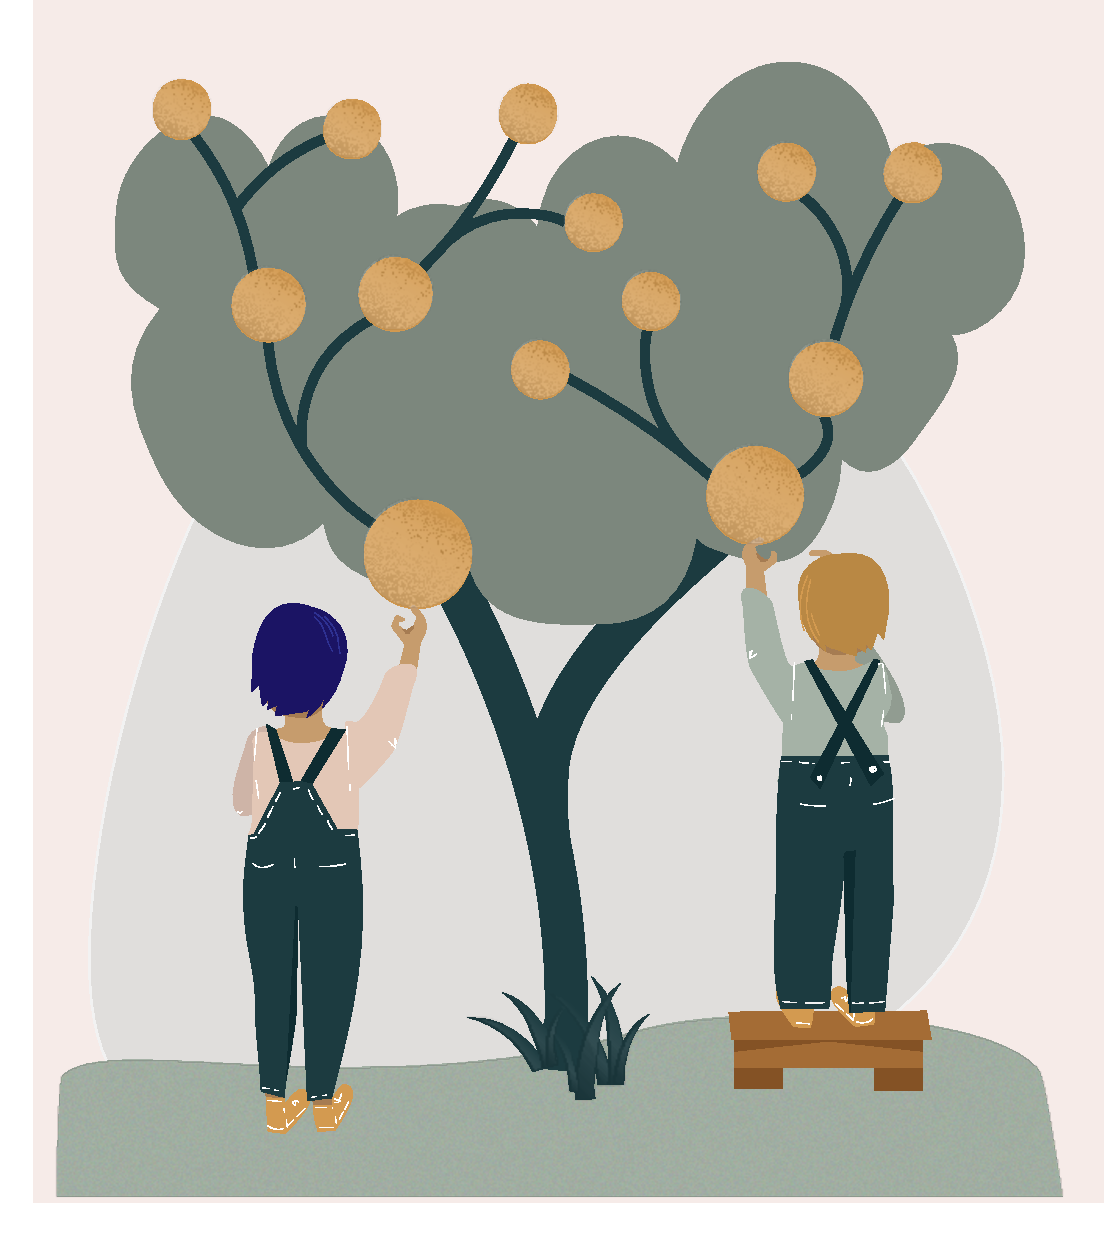
\includegraphics[keepaspectratio,alt={Equidade}]{img/equity.pdf}}
\caption{Equidade}
\end{figure}

Por outro lado, há também critérios que não são fundamentos
justificáveis para tratar pessoas de modo diferente. Em geral,
consideramos injusto dar tratamento especial a indivíduos com base em
idade, sexo, raça ou preferências religiosas. Em outras palavras: o que
é discriminação?

\begin{nota}[Tipos de justiça]

\textbf{Justiça distributiva} é a medida em que as instituições da
sociedade asseguram que benefícios e ônus sejam distribuídos entre seus
membros de maneira justa.

\textbf{Justiça retributiva} é a medida em que as punições são justas.
Em geral, as punições são consideradas justas na medida em que levam em
conta critérios relevantes, como a gravidade do crime e a intenção do
criminoso, e descartam critérios irrelevantes, como a raça.

\textbf{Justiça compensatória} é a medida em que as pessoas são
justamente compensadas por seus danos por aqueles que as prejudicaram; a
compensação justa é proporcional à perda infligida. É precisamente esse
tipo de justiça que está em jogo nos debates sobre danos à saúde de
trabalhadores em minas de carvão. Alguns argumentam que os donos das
minas deveriam compensar os trabalhadores cuja saúde foi arruinada.
Outros argumentam que os trabalhadores assumiram voluntariamente esse
risco ao escolher o emprego nas minas.

\end{nota}

\subsection{III. Discriminação e
vieses}\label{iii.-discriminauxe7uxe3o-e-vieses}

Nesta seção estudaremos a discriminação e o modo como práticas
discriminatórias podem se manifestar por meio da inteligência
artificial. O viés tornou-se recentemente a questão prototípica da ética
da IA, já que a esperança de que a formalidade exata dos algoritmos os
tornasse imunes à parcialidade revelou-se dolorosamente falsa. Primeiro,
veremos três exemplos de sistemas algorítmicos que nos ajudarão a
analisar discriminação e viés em IA.

\paragraph{\texorpdfstring{Exemplo 1: \emph{word embeddings}
(\href{https://arxiv.org/abs/1607.06520}{Bolukbasi et
al.})}{Exemplo 1: word embeddings (Bolukbasi et al.)}}\label{exemplo-1-word-embeddings-bolukbasi-et-al.}

Vetores de palavras (\emph{word embeddings}) são uma forma de estrutura
de dados usada em aplicações de processamento de linguagem natural (IA
capaz de compreender uma língua, como o inglês). São produzidos
vasculhando textos e registrando quais palavras ocorrem juntas com
frequência. As associações produzidas funcionam como uma espécie de
dicionário para sistemas de IA, capturando relações semânticas do tipo
``homem'' está para ``rei'' assim como ``mulher'' está para ``rainha''.
Bolukbasi et al.~constataram que, sem grande surpresa, esse tipo de
associação tende a codificar relações conceituais culturalmente
disseminadas, mas consideradas discriminatórias. Por exemplo: ``mãe''
está para ``enfermeira'' assim como ``pai'' está para ``médico''.

\begin{figure}
\centering
\pandocbounded{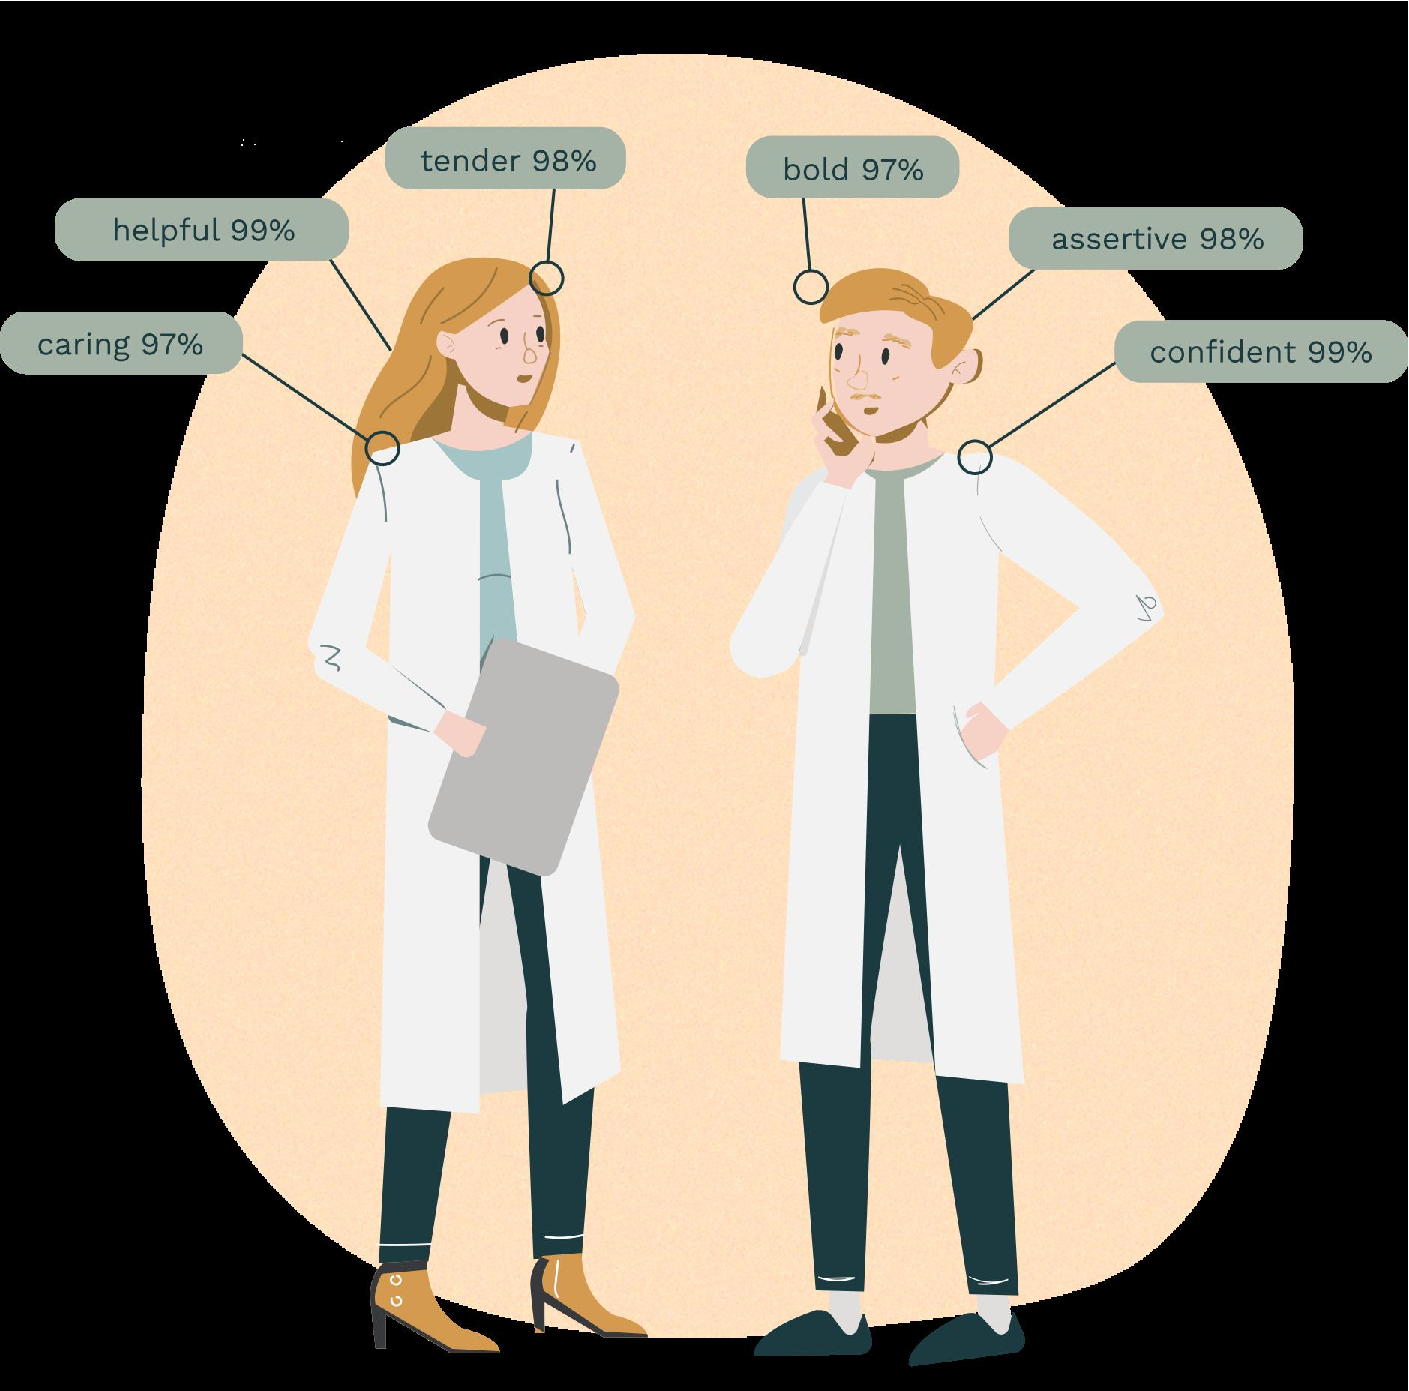
\includegraphics[keepaspectratio,alt={Viés em vetores de palavras}]{img/bias.pdf}}
\caption{Viés em vetores de palavras}
\end{figure}

\paragraph{\texorpdfstring{Exemplo 2: o algoritmo de recrutamento da
Amazon
(\href{https://www.reuters.com/article/us-amazon-com-jobs-automation-insight/amazon-scraps-secret-ai-recruiting-tool-that-showed-bias-against-women-idUSKCN1MK08G}{Dastin,
2018})}{Exemplo 2: o algoritmo de recrutamento da Amazon (Dastin, 2018)}}\label{exemplo-2-o-algoritmo-de-recrutamento-da-amazon-dastin-2018}

Em 2014, a Amazon começou a desenvolver um sistema interno de IA para
agilizar seu processo de recrutamento. Usando os currículos de
candidatos anteriores como dados de treinamento, o sistema analisaria os
currículos recebidos e classificaria os candidatos para avaliação
posterior. Muito rapidamente, porém, descobriu-se que o sistema
classificava candidatos a vagas técnicas de maneira enviesada por
gênero.

Constatou-se que o sistema penalizava currículos que indicassem que a
candidata era mulher. Isso incluía menções a coisas como participação em
um clube feminino de xadrez ou formação numa faculdade exclusivamente
feminina. Segundo relatos, a Amazon tentou remover o viés do sistema,
mas acabou descartando o projeto inteiro. O sistema nunca foi usado em
processos reais de recrutamento.

\paragraph{\texorpdfstring{Exemplo 3: pontuação de crédito
(\href{https://algorithmwatch.org/en/automating-society-2019/finland/}{Rutkenstein
\& Velkova,
2019})}{Exemplo 3: pontuação de crédito (Rutkenstein \& Velkova, 2019)}}\label{exemplo-3-pontuauxe7uxe3o-de-cruxe9dito-rutkenstein-velkova-2019}

Em 2018, o tribunal finlandês de não discriminação e igualdade julgou um
caso em que uma solicitação de crédito ao consumidor foi negada
automaticamente por métodos estatísticos. A instituição de crédito Svea
Ekonomi avaliou automaticamente a capacidade de crédito de um indivíduo
no âmbito de sua compra online de materiais de construção, para a qual
ele buscava crédito. A decisão foi contestada, e o tribunal concluiu que
``a idade do solicitante, seu gênero masculino, o finlandês como língua
materna e a residência em área rural foram todos fatores que
contribuíram para um caso de discriminações múltiplas, resultando na
decisão de não conceder o empréstimo.'' O tribunal observou que, se o
solicitante fosse mulher ou falante de sueco, o crédito teria sido
concedido.

\paragraph{O que é discriminação?}\label{o-que-uxe9-discriminauxe7uxe3o}

Primeiro, é importante notar que a palavra discriminação pode ser usada
num sentido moralmente neutro (``você consegue discriminar entre estas
duas cores?''). Ao longo desta seção, referimo-nos ao sentido moralmente
carregado do termo. Mas quando a discriminação é moralmente suspeita?
Pode parecer uma pergunta boba. Afinal, a maioria concordaria que temos
um senso intuitivo bastante claro do que seja discriminação. Ao ouvir o
exemplo dos vetores de palavras acima, não temos dificuldade em apontar
a associação ofensiva e declarar: ``isto é discriminatório!'' Colocar em
palavras o que a torna discriminatória, contudo, revela-se uma tarefa
escorregadia. Comecemos, então, escrevendo nossas intuições, e vejamos
aonde isso leva:

\begin{definicao}[Definição 1: discriminação]

Discriminação é uma diferença de tratamento de indivíduos com base em
sua pertença a um grupo.

\end{definicao}

Como essa definição se sai ao capturar nosso senso de discriminação? As
palavras que fazem o trabalho aqui são ``diferença'' e ``grupo''. Ou
seja, a discriminação é algo comparativo, e as unidades de comparação
são grupos diferentes (ou, antes, agrupamentos), ou indivíduos que
pertencem a eles. É um bom começo, mas analisemos onde essa definição
traça a linha. O que fica dentro e o que fica de fora?

Considere, por exemplo, as carteiras de motorista. Na Finlândia, elas
são emitidas pela polícia mediante a conclusão de certa carga de
treinamento prático e teórico, além de um exame. Assim, as carteiras são
emitidas com base no mérito individual. Ainda assim, em geral achamos
sensato que pessoas com deficiência visual severa sejam excluídas do
processo por completo, e não consideramos isso discriminatório no
sentido moral. Afinal, dirigir seria praticamente impossível de qualquer
modo. Precisamos, portanto, incluir algum sentido de nocividade em nossa
definição.

Considere, então, um café que só atende pessoas de camisa verde. Isso é
definitivamente tratamento diferenciado com base em pertencimento a um
grupo, e conduz a algum tipo de prejuízo, mas também não consideraríamos
isso discriminação em sentido moral. Poderíamos achar a política
estranha, mas não moralmente problemática. Assim, não é apenas o
pertencimento a um grupo que nos interessa, mas \emph{quais} grupos.

\begin{definicao}[Definição 2: discriminação]

Discriminação é tratamento diferenciado com base em pertencimento
percebido a um grupo socialmente saliente, que causa dano social
(\href{https://oxford.universitypressscholarship.com/view/10.1093/acprof:oso/9780199796113.001.0001/acprof-9780199796113}{Lippert-Rasmussen,
2014}).

\end{definicao}

A ``saliência social'' é o que identifica quais características são
moralmente relevantes em casos de discriminação. Mas o que isso
significa? Segundo Lippert-Rasmussen, uma característica é socialmente
saliente se for importante para a estrutura das interações sociais em
múltiplos contextos. Ou seja, o que se considera classificação
socialmente saliente é uma questão historicamente contingente: numa
linha temporal alternativa, em que usar camisa verde fosse
invariavelmente questão de importância social, influindo no tipo de
dignidade, oportunidades ou status conferidos a uma pessoa (se fosse
vestimenta religiosa, por exemplo), o caso do café acima poderia
perfeitamente contar como discriminação.

Reconhecer a discriminação em sentido moral não é, portanto,
simplesmente reconhecer discrepâncias de tratamento entre agrupamentos
arbitrários. Exige, antes, contextualizar o tratamento desigual na
história das práticas opressivas ou valorativas da sociedade e nos
agrupamentos que ela torna salientes. Por exemplo, a Carta dos Direitos
Fundamentais da União Europeia lista as seguintes características como
moralmente pertinentes em casos de discriminação: sexo, raça, cor,
origem étnica ou social, características genéticas, língua, religião ou
convicções, opiniões políticas ou outras, pertença a uma minoria
nacional, propriedade, nascimento, deficiência, idade e orientação
sexual.

\subsubsection{Os danos --- o que são?}\label{os-danos-o-que-suxe3o}

Refletindo sobre os dois exemplos acima, a condição de saliência social
está claramente satisfeita em ambos. Gênero é uma categoria que
historicamente sempre estruturou a interação social. E quanto ao dano?
Um caso é mais claro que o outro: perder uma oportunidade de emprego por
razões alheias à adequação ao cargo é claramente um dano. No caso dos
vetores de palavras, qualquer dano que ocorra é mais difícil de
localizar. Ao menos, não conseguimos apontar diretamente uma
oportunidade perdida, um serviço recusado ou um bem negado. Ainda assim,
em casos assim um dano é instaurado. Para captá-lo, precisamos
compreender a diferença entre danos \textbf{alocativos} e
\textbf{representacionais}, como apresentados em
\href{https://www.youtube.com/watch?v=fMym_BKWQzk}{Crawford, 2017}.

\paragraph{Danos alocativos}\label{danos-alocativos}

Danos alocativos são situações em que um indivíduo fica em pior situação
quanto aos recursos disponíveis para ele. Aqui, ``recursos'' devem ser
entendidos amplamente: não apenas comida, carros, celulares e outros
bens materiais, mas também os serviços e as oportunidades oferecidos. Um
salário menor pelo mesmo trabalho é definitivamente um dano alocativo.
Mas também o é negar a oportunidade de uma entrevista de emprego com
base no gênero, ou negar crédito com base nele.

Até abstrações como o risco podem ser objeto de danos alocativos.
\href{http://arxiv.org/abs/1902.11097}{Wilson, Hoffman e Morgenstern
(2019)} constataram que algoritmos de detecção de objetos são piores em
reconhecer figuras de tom de pele escuro do que de tom claro. As
pesquisadoras Joy Buolamwini e Timnit Gebru também mostraram que
algoritmos de reconhecimento facial são notavelmente piores em
reconhecer rostos de pessoas racializadas
(\href{http://proceedings.mlr.press/v81/buolamwini18a/buolamwini18a.pdf}{Buolamwini
e Gebru, 2018}). Isso significa que carros autônomos podem ter mais
probabilidade de atropelar uma pessoa negra do que uma branca. Ora, dado
que causar dano corporal é claramente um dano, pode-se argumentar que um
dano já ocorreu mesmo antes de tais acidentes acontecerem: a
distribuição desigual do risco é, ela própria, um dano alocativo à parte
prejudicada.

\paragraph{Danos representacionais}\label{danos-representacionais}

Danos representacionais são aqueles que não dizem respeito à
distribuição de bens, e sim à representação de grupos e indivíduos. Essa
classe inclui danos como denegrição, estereotipagem, falha de
reconhecimento (\emph{misrecognition}) e \emph{exnominação}. Exnominação
é um termo originado dos estudos de mídia e designa a prática pela qual
certa categoria ou modo de ser é enquadrado como norma por não receber
nome, ou por não ser especificado como categoria em si (por exemplo,
``atleta'' \emph{vs.} ``atleta feminina'').

Danos representacionais afetam as narrativas que construímos sobre os
grupos sociais relevantes. Ao amplificar visões estereotipadas, degradar
o status social de indivíduos e enquadrar certos modos de ser como o
padrão, os danos representacionais fabricam as justificativas infundadas
para práticas opressivas.

Com o conceito de danos representacionais, somos capazes de identificar
as associações de palavras enviesadas por gênero como discriminatórias,
ainda que elas próprias não sejam um exemplo de distribuição de recursos
no sentido dos danos alocativos.

\subsubsection{Como o viés surge?}\label{como-o-viuxe9s-surge}

\begin{quote}
\emph{``Todo dado é dado histórico: produto de um tempo, de um lugar, de
um clima político, econômico, técnico e social. Se você não está
considerando por que seus dados existem, e por que outros conjuntos de
dados não existem, você está fazendo ciência de dados errado.''}

\href{https://www.youtube.com/watch?v=4yYytLUViI4}{Melissa Terras
(2019)}
\end{quote}

\begin{definicao}[Três sentidos de "viés"]

Na \textbf{estatística}: discrepância entre a estatística de uma amostra
e a estatística verdadeira da população.

Na \textbf{ciência cognitiva}: um modo de raciocínio que provavelmente
produz resultado incorreto ou distorcido.

Na \textbf{justiça social}: uma discrepância moralmente suspeita no
tratamento de pessoas.

\end{definicao}

Até aqui conseguimos encontrar uma definição razoável de discriminação e
temos ao menos dois exemplos concretos de sistemas de IA participando
dela. Em ambos, a prática discriminatória decorre de vieses no próprio
sistema. Portanto, se quisermos lidar com a questão, temos algumas
perguntas a responder. Como sistemas de IA se tornam enviesados? Como
podemos medir se um sistema é enviesado? Como podemos corrigi-lo?

Nesta seção, veremos como práticas discriminatórias se retroalimentam.
Ou seja, uma IA enviesada não é apenas uma questão técnica, mas
resultado de uma história de práticas sociais. Podemos detectar quando
nossos sistemas amplificam essas tendências discriminatórias e, melhor
ainda, como podemos interromper o ciclo? Veremos três maneiras pelas
quais o viés entra num sistema:

\paragraph{1) Amostra não
representativa}\label{amostra-nuxe3o-representativa}

O modo mais evidente pelo qual o viés entra num sistema é por um
conjunto de dados não representativo. Ou seja, os dados que alimentam o
sistema de aprendizado não são um retrato fiel do mundo em geral. Não
surpreende que, ao manipular o modo como o aprendiz vê o mundo ---
amplificando algumas instâncias de fenômenos e suprimindo outras ---, o
sistema aprenda um modelo distorcido.

Por exemplo, a capacidade de reconhecer pessoas é distribuída
desigualmente entre grupos étnicos em muitos sistemas de reconhecimento
facial. O resultado é que o sistema de classificação de imagens do
Google, por exemplo, chegou a rotular pessoas negras como gorilas
(\href{https://www.theguardian.com/technology/2015/jul/01/google-sorry-racist-auto-tag-photo-app}{Kasperkevic,
2015}).

Uma razão para isso, segundo
\href{http://proceedings.mlr.press/v81/buolamwini18a/buolamwini18a.pdf}{Buolamwini
e Gebru (2018)}, é que muitos conjuntos de dados populares de rostos têm
distribuição muito pobre de exemplos entre diferentes gêneros e etnias.
Ou seja, a visão dos rostos do mundo fornecida aos sistemas de
aprendizado é inegavelmente branca e masculina, e muito pouco
representativa da verdadeira distribuição de rostos no mundo. Às vezes
isso é tecnicamente chamado de disparidade de tamanho amostral, e leva a
sistemas enviesados porque o algoritmo de aprendizado despreza
subpopulações mal representadas para alcançar maior capacidade preditiva
sobre a maioria do conjunto de dados.

\paragraph{2) Viés de rótulo}\label{viuxe9s-de-ruxf3tulo}

``Deixe os dados falarem por si'', diz o ditado. É um bom pensamento,
mas a verdade infeliz é que os dados não têm voz própria. Os dados só
falam por meio de nossas interpretações --- e com frequência essas
interpretações são difíceis de fazer. Isso é especialmente verdadeiro em
situações em que há discrepância entre o que está sendo medido e o que
está sendo investigado.

Por exemplo, prever crimes é uma tarefa que, se bem-feita, interessaria
a tribunais, polícias e cidadãos igualmente. Infelizmente, crime é algo
difícil de medir e, portanto, bons conjuntos de dados são difíceis de
produzir. O que conseguimos medir são coisas a que temos acesso
informacional, como prisões e condenações. A esperança é que esses
substitutos (\emph{proxies}) se correlacionem bem com a quantidade de
crime numa população. Além disso, deveríamos desejar que se
correlacionem igualmente bem entre grupos socialmente salientes dentro
dela.

A verdade infeliz é que prisões dificilmente são um substituto neutro
para crime. Podem dar boa noção do crime geral numa população, mas não
se generalizam bem entre agrupamentos. Nos Estados Unidos, pessoas
negras podem ter probabilidade muito maior de serem presas por acusações
relacionadas a drogas do que pessoas brancas
(\href{https://www.ncbi.nlm.nih.gov/pmc/articles/PMC6050822/}{Ferrer \&
Connolly, 2018}), por exemplo. Isso não significa que pessoas negras
tenham mais probabilidade de cometer crimes de drogas, apenas que têm
mais probabilidade de serem flagradas, presas e registradas fazendo
isso. Assim, quaisquer inferências sobre crime a partir desses dados
necessariamente repetirão e reforçarão as injustiças que produziram os
próprios dados.

\paragraph{3) Desconhecimento cultural}\label{desconhecimento-cultural}

Embora ``IA'' e ``aprendizado de máquina'' (\emph{machine learning})
evoquem uma imagem de autonomia maquínica, na realidade grande
quantidade de trabalho --- trabalho humano --- é necessária para tornar
sistemas de IA reais. Assim, o comportamento de sistemas de IA não pode
ser compreendido olhando apenas para o algoritmo e para os dados que
entram nele. Escolhas são feitas no trabalho de implantação,
interpretação, projeto e manutenção envolvido na IA, e às vezes essas
escolhas criam vieses no sistema.

Um dos exemplos mais claros disso está nos modos pelos quais os dados
são ``limpos'', envolvendo decisões sobre o que é sinal real em oposição
a ruído incômodo. Essa é uma tarefa por vezes vista como faxina e,
portanto, como algo que não faz parte do núcleo do negócio da IA --- e
acontece despercebida em muitas etapas do processo. Por exemplo, ao
coletar dados em formulários web, chama-se sanitização de entrada.

\begin{tecnica}[O problema dos nomes]

Um bom exemplo é a coleta de nomes. Para impedir que dados falsos entrem
no sistema, criam-se certas restrições sobre como os nomes devem ser.
Por exemplo, às vezes se supõe que nomes consistem em prenomes e um
sobrenome. Às vezes se supõe que nomes contêm apenas letras de A a Z. Às
vezes se supõe que nomes sempre têm mais de duas letras.

Essas podem ser suposições razoáveis no contexto cultural limitado dos
projetistas e programadores, mas na realidade os nomes são extremamente
diversos. Nenhuma forma universal de nome pode realmente ser dada e, se
alguém quiser ser verdadeiramente inclusivo, todos os campos de nome em
formulários web deveriam ser caixas de texto de comprimento arbitrário
que aceitem qualquer tipo de caractere. Sem compreensão cultural
diversa, o sistema pode ser projetado, sem intenção, de modo a deixar de
fora grandes grupos de pessoas que não se enquadram nos padrões
culturais dominantes.

\end{tecnica}

O viés pode, portanto, entrar num sistema de muitas maneiras diferentes,
e as acima são apenas alguns exemplos dos mecanismos em jogo. O ponto
importante aqui é que, ao analisar sistemas de IA em busca de injustiça,
não basta olhar para os algoritmos. A injustiça pode surgir por razões
históricas, culturais, de projeto, de gestão de dados ou de implantação
--- e, portanto, todo o processo de desenvolvimento de IA deve estar sob
escrutínio.

\subsection{IV. Removendo o viés}\label{iv.-removendo-o-viuxe9s}

Como, então, tornamos sistemas de IA mais justos e menos enviesados? Não
há panaceia para o viés --- em parte por causa das muitas formas pelas
quais ele pode se manifestar, em parte porque não existe uma definição
única de resultado algoritmicamente justo. Ainda assim, podemos examinar
algumas das situações acima e pensar em como os problemas de justiça
poderiam potencialmente ter sido tratados.

Começando pelo exemplo do algoritmo sexista de recrutamento, podemos
localizar a origem do viés nas práticas históricas de recrutamento que
produziram os dados de treinamento, e na suposição de que práticas
passadas fornecem base normativa para práticas futuras (isto é:
``devemos contratar esta pessoa porque já contratamos pessoas como ela
antes''). Vemos que as questões de fundo estão inexoravelmente ligadas à
cultura da empresa e até à cultura de trabalho mais ampla do setor de
tecnologia, bem como a um raciocínio moralmente suspeito (lembre-se da
guilhotina de Hume, no capítulo 1). São problemas que exigem grandes
deslocamentos culturais e reformas estruturais, e é improvável que sejam
resolvidos por soluções tecnológicas.

\paragraph{Anticlassificação}\label{anticlassificauxe7uxe3o}

Ainda assim, poder-se-ia tentar salvar o que for possível do conjunto de
dados e ver se ele poderia ficar ao menos menos enviesado. Um conserto
técnico comum sobre o conjunto de dados chama-se anticlassificação, ou
remoção explícita das variáveis protegidas. Isso significa apagar
informações como gênero ou etnia, e seus substitutos, dos dados. Aqui,
substitutos são características fortemente correlacionadas com as
características protegidas. Como no caso do algoritmo de recrutamento
mencionado antes, se o currículo de uma pessoa contém referências a
licença-maternidade ou a uma faculdade feminina, o algoritmo ainda
poderia fazer previsões marcadas por gênero mesmo que a variável
explícita de gênero seja omitida.

Isso pode contribuir em certa medida para reduzir o viés no sistema, mas
se é eficaz em algum cenário específico precisa ser verificado por
testes e auditoria. Corbett-Davies e Goel (2018) mostraram que a
anticlassificação pode até ser prejudicial à justiça em certas
situações, nas quais características têm poder preditivo diferente entre
grupos sociais. Uma ilustração são os sintomas de infarto: pesquisas
mostraram que infartos se apresentam de modo muito diferente em
pacientes mulheres e homens. Os sintomas que a maioria sabe procurar,
por exemplo dor torácica do lado direito, são muito mais comuns em
pacientes homens do que mulheres. Assim, um aplicativo em que se pudesse
verificar ``estou tendo um infarto?'' provavelmente daria resultados
muito errados se não levasse em conta o sexo do paciente.

\paragraph{Reamostragem}\label{reamostragem}

Em casos como o do algoritmo de reconhecimento facial pesquisado por
Buolamwini e Gebru, em que o viés é produzido por disparidade de tamanho
amostral, a reamostragem é uma forma possível de abordar o problema.
Isso pode significar usar apenas uma porção menor do conjunto de dados,
que tenha melhor distribuição de exemplos entre todos os agrupamentos
sociais relevantes. Outra forma de reamostrar é produzir exemplos
sintéticos dos grupos sub-representados (Chawla et al., 2002).
Novamente, se isso funciona é questão de verificação caso a caso. Pode
ser que o conjunto de dados esteja tão desequilibrado que não haja como
corrigi-lo, a não ser criando um novo do zero. Além disso, num caso tão
sensível e de alto risco como o reconhecimento facial, não é dado que o
sistema será ético, justo e não discriminatório mesmo que a
classificação seja não enviesada e o conjunto de dados igualmente
representativo. Abordaremos isso na próxima seção mas, em termos de
tornar a IA justa, às vezes a única maneira de fazê-lo é não desenvolver
aquela IA em primeiro lugar.

\paragraph{Discriminação para além do
viés}\label{discriminauxe7uxe3o-para-aluxe9m-do-viuxe9s}

O importante a lembrar aqui é que discriminação não é o mesmo que viés
sistemático. O viés em sistemas de IA é causa bastante evidente de
práticas discriminatórias e, por sua natureza quantificável, encaixa-se
facilmente no mundo conceitual da pesquisa técnica em IA. Talvez seja
por isso que o salto conceitual da discriminação para o viés seja feito
com tanta frequência.

Ainda assim, sistemas de IA podem participar de práticas
discriminatórias que não decorrem de viés no próprio sistema.
Precisamos, antes, expandir nosso objeto de investigação das minúcias do
modelo de IA para todo o sistema de instituições do qual ele participa.

\begin{nota}[Quando o problema não é a acurácia]

No início de 2018, pesquisadores da Stanford Graduate School of Business
publicaram um artigo detalhando um sistema de aprendizado profundo
(\emph{deep learning}) capaz de distinguir entre homens gays e
heterossexuais com acurácia de 81\% a partir de uma única foto do rosto.
Os achados foram controversos, no mínimo, e por muitas razões
diferentes. Críticos levantaram preocupações sobre a ressurreição da
pseudociência da fisiognomia, que tem conexão profundamente enraizada
com injustiças racistas históricas. Houve também suspeitas de que o
sistema, em vez de captar sutis marcadores genéticos como se alegava, na
verdade estivesse rastreando o modo como as pessoas tendem a se arrumar
e a tirar fotos de si mesmas.

Além disso, esse sistema de IA opera claramente numa área eticamente
nebulosa quanto a privacidade, autodeterminação e, evidentemente,
discriminação. Deixando de lado as outras preocupações por ora, como a
discriminação funciona aqui? Claramente o viés de classificação não é o
elemento discriminatório: não é eticamente relevante para nós se o
estimador é mais acurado em prever homossexualidade em alguns grupos do
que em outros. A característica eticamente relevante do sistema é que,
independentemente de sua acurácia, ele possibilita diretamente
tratamento diferenciado com base em agrupamento social percebido.

\end{nota}

Não é preciso detalhar exemplos de usos maliciosos de sistemas como o
descrito acima, pois sua possibilidade deve ser óbvia a todos. Deixando
de lado os usos diretamente maliciosos, podemos imaginar a integração de
tal tecnologia, por exemplo, à maquinaria de publicidade personalizada
online composta por redes sociais, processadores de dados,
influenciadores de tendências e comerciantes globais. Mesmo que a IA
classificadora seja, por todos os padrões técnicos, justa e não
enviesada, ela condiciona a publicidade online de bens ao princípio
discriminatório de que a orientação sexual presumida é razão válida para
tratar pessoas de modo diferente.

Isso nos leva a um ponto importante para quem considera a ética dos
sistemas de IA: cuidado com a armadilha do reducionismo! Ou seja,
devemos evitar reduzir o conceito de ética a valores simplificados,
quantificados e de atalho, como ``ausência de viés''. Como sistemas de
IA participam de processos muito mais complexos do que aquilo que o
próprio sistema faz, a ética não pode ser medida apenas olhando os
valores de entrada e de saída do algoritmo.

Em suma: \textbf{justo não significa ético}.

\begin{reflexao}[Exercícios desta seção]

O material original traz aqui dois questionários interativos. As
perguntas não constam do repositório de origem --- ficam no banco de
dados da plataforma. Os exercícios correspondentes devem ser redigidos
em \texttt{exercicios/capitulo06-exercicios.md}.

\end{reflexao}

\subsection{Referências}\label{referuxeancias}

Bolukbasi, T., Chang, K.-W., Zou, J., Saligrama, V., \& Kalai, A.
(2016). Man is to Computer Programmer as Woman is to Homemaker?
Debiasing Word Embeddings. \url{https://arxiv.org/abs/1607.06520}

Buolamwini, J., \& Gebru, T. (2018). Gender Shades: Intersectional
Accuracy Disparities in Commercial Gender Classification. \emph{PMLR}
81.
\url{http://proceedings.mlr.press/v81/buolamwini18a/buolamwini18a.pdf}

Chawla, N. V., et al.~(2002). SMOTE: Synthetic Minority Over-sampling
Technique.

Corbett-Davies, S., \& Goel, S. (2018). The Measure and Mismeasure of
Fairness.

Crawford, K. (2017). The Trouble with Bias. \emph{NIPS 2017 Keynote}.

Dastin, J. (2018). Amazon scraps secret AI recruiting tool that showed
bias against women. \emph{Reuters}.

Ferrer, B., \& Connolly, J. M. (2018). Racial Inequities in Drug
Arrests.

Kasperkevic, J. (2015). Google says sorry for racist auto-tag in photo
app. \emph{The Guardian}.

Lippert-Rasmussen, K. (2014). \emph{Born Free and Equal?} Oxford
University Press.

Rawls, J. (1971). \emph{A Theory of Justice}. Harvard University Press.

Rutkenstein, M., \& Velkova, J. (2019). Automating Society: Finland.
\emph{AlgorithmWatch}.

Terras, M. (2019). Palestra.
\url{https://www.youtube.com/watch?v=4yYytLUViI4}

Wilson, B., Hoffman, J., \& Morgenstern, J. (2019). Predictive Inequity
in Object Detection. \url{http://arxiv.org/abs/1902.11097}

\begin{center}\rule{0.5\linewidth}{0.5pt}\end{center}

\begin{licenca}

\textbf{Material original:} \emph{Ethics of AI}, um curso online
gratuito da Universidade de Helsinque. Professores responsáveis:
Anna-Mari Rusanen e Jukka K. Nurminen. Demais contribuintes principais:
Santeri Räisänen, Sasu Tarkoma e Saara Halmetoja. Disponível em
\url{https://ethics-of-ai.mooc.fi/}.

\textbf{Esta versão:} tradução e adaptação para o português brasileiro
realizada por José Lucas Lira Bizil, Fernando Mazzeto Lisboa Lima e
Matheus da Silva Fernandes, no âmbito do Programa CiberExt 26-29
(FEELT38103), Universidade Federal de Uberlândia, 2026. Esta é uma obra
derivada; os autores originais não a revisaram nem a endossam.

\textbf{Licença:} Creative Commons
Atribuição-NãoComercial-CompartilhaIgual 4.0 Internacional (CC BY-NC-SA
4.0) ---
\url{https://creativecommons.org/licenses/by-nc-sa/4.0/deed.pt-br}.

\end{licenca}

\end{document}
